%%%%%%%%%%%%%%%%%%%%%%%%%%%%%%%%%%%%%%%%%
% Formal Book Title Page
% LaTeX Template
% Version 2.0 (23/7/17)
%
% This template was downloaded from:
% http://www.LaTeXTemplates.com
%
% Original author:
% Peter Wilson (herries.press@earthlink.net) with modifications by:
% Vel (vel@latextemplates.com)
%
% License:
% CC BY-NC-SA 3.0 (http://creativecommons.org/licenses/by-nc-sa/3.0/)
% 
% This template can be used in one of two ways:
%
% 1) Content can be added at the end of this file just before the \end{document}
% to use this title page as the starting point for your document.
%
% 2) Alternatively, if you already have a document which you wish to add this
% title page to, copy everything between the \begin{document} and
% \end{document} and paste it where you would like the title page in your
% document. You will then need to insert the packages and document 
% configurations into your document carefully making sure you are not loading
% the same package twice and that there are no clashes.
%
%%%%%%%%%%%%%%%%%%%%%%%%%%%%%%%%%%%%%%%%%

%----------------------------------------------------------------------------------------
%	PACKAGES AND OTHER DOCUMENT CONFIGURATIONS
%----------------------------------------------------------------------------------------

\documentclass[11pt]{article} % A4 paper size, default 11pt font size and oneside for equal margins

\usepackage[a4paper, margin=1in]{geometry}

\usepackage[utf8]{inputenc} % Required for inputting international characters
\usepackage[T1]{fontenc} % Output font encoding for international characters
\usepackage{fouriernc} % Use the New Century Schoolbook font

\usepackage[]{todonotes}
\usepackage{verbatim}
\usepackage{parskip}
\usepackage[acronym]{glossaries}
\usepackage{eucal}
\usepackage{bm}
\usepackage{rotating}
%\usepackage{hyperref}

\usepackage{physics}
% \usepackage{amsmath}
\usepackage{tikz}
\usepackage{mathdots}
% \usepackage{yhmath}
\usepackage{cancel}
\usepackage{color}
\usepackage{siunitx}
\usepackage{array}
\usepackage{multirow}
% \usepackage{amssymb}
\usepackage{gensymb}
\usepackage{tabularx}
\usepackage{booktabs}
\usepackage{wrapfig}
\usetikzlibrary{fadings}
\usetikzlibrary{patterns}
\usetikzlibrary{shadows.blur}
\usetikzlibrary{shapes}

\usepackage[backend=bibtex]{biblatex}
\addbibresource{report.bib}


\newcommand{\e}[2]{#1\cdot 10^{#2}}

% 
%----------------------------------------------------------------------------------------
%	TITLE PAGE
%----------------------------------------------------------------------------------------

\begin{document} 
    \begin{titlepage} % Suppresses headers and footers on the title page

        \centering % Centre everything on the title page
        
        \scshape % Use small caps for all text on the title page
        
        \vspace*{\baselineskip} % White space at the top of the page
        
        %------------------------------------------------
        %	Title
        %------------------------------------------------
        
        \rule{\textwidth}{1.6pt}\vspace*{-\baselineskip}\vspace*{2pt} % Thick horizontal rule
        \rule{\textwidth}{0.4pt} % Thin horizontal rule
        
        \vspace{0.75\baselineskip} % Whitespace above the title
        
        {\LARGE PRACTICAL ASSIGNMENT AE4-301P} % Title
        
        \vspace{0.75\baselineskip} % Whitespace below the title
        
        \rule{\textwidth}{0.4pt}\vspace*{-\baselineskip}\vspace{3.2pt} % Thin horizontal rule
        \rule{\textwidth}{1.6pt} % Thick horizontal rule
        
        \vspace{2\baselineskip} % Whitespace after the title block
        
        %------------------------------------------------
        %	Subtitle
        %------------------------------------------------
        
        Exercise Automatic Flight Control System Design
        % Subtitle or further description
        
        \vspace*{3\baselineskip} % Whitespace under the subtitle
        
        %------------------------------------------------
        %	Editor(s)
        %------------------------------------------------
        
        \vspace{0.5\baselineskip} % Whitespace before the editors
        
        {\scshape\Large Aaron de Windt --- 4134249} % Editor list
        
        \vspace{0.5\baselineskip} % Whitespace below the editor list
        
        \textit{Delft University of Technology \\ Delft} % Editor affiliation
        
        \vfill % Whitespace between editor names and publisher logo
        
        %------------------------------------------------
        %	Publisher
        %------------------------------------------------
        
        % \plogo % Publisher logo
        
        \vspace{0.3\baselineskip} % Whitespace under the publisher logo
        
        2021 % Publication year
        
        % {\large publisher} % Publisher

    \end{titlepage}

%----------------------------------------------------------------------------------------

    \tableofcontents
    
    \newpage

    \section{Flight condition}
Based on the rules given in the assignment the chosen set of flight conditions are,

\begin{equation*}
    Altitude = 40000ft \qquad  Velocity=300ft/s
\end{equation*}

    \section{Trim and linearisation}

\subsection{Trimming}
The first step when designing the control system of an aircraft is to study the behavior of the aircraft due to control inputs or external disturbances from an equilibrium condition. If the aircraft we're not to be in equilibrium, deviation from the initial conditions would occur that are unrelated to the control inputs making the analysis more difficult.

In the case of an aircraft this equilibrium condition is known as a trimmed flight condition. In order to determine the trimmed flight condition the states and inputs much be chosen such that the linear- and angular-accelerations are zero. For this assignment this is done by minimizing the following cost function.

\begin{equation}
    \label{eq:trim_cost}
    cost = W_{h}\dot{h}^2 + 
           W_{\phi}\dot{\phi}^2 +
           W_{\theta}\dot{\theta}^2 + 
           W_{\psi}\dot{\psi}^2 +
           W_{V}\dot{V}^2 + 
           W_{\alpha}\dot{\alpha}^2 + 
           W_{\beta}\dot{\beta}^2 + 
           W_{P}\dot{P}^2 +
           W_{Q}\dot{Q}^2 +
           W_{R}\dot{R}^2
\end{equation}

The weights can be used to select which states need to be optimized to zero since this can vary with the chosen flight conditions. All the flight states in the cost function are squared, which is what allows the trim condition to be found by minimizing the the cost function. Once the cost function returns zero, the trimmed flight condition states and inputs have been found.

Performing the trimming procedure for 5 iterations in level flight for both flight conditions and both the high and low fidelity models yields the following final values for the cost function.

\begin{center}
    \begin{tabular}{ r | c | c }
                               & high fidelity & low fidelity \\ \hline \hline
     Assigned flight condition & $0.0506$ & $4.2997\cdot10^{-29}$ \\  
     APA flight condition      & $7.1856\cdot10^{-6}$ & $5.1572\cdot10^{-29}$    
    \end{tabular}
\end{center}

The results for the low fidelity models are smaller than the machine epsilon $2.2204\cdot10^{-16}$ of the computer used to calculate these, so it's safe to assume the trimmed flight condition has been successfully found. 

The final cost for the high fidelity model are higher. The results for the APA flight conditions are in the order of $10^{-6}$ and for the assigned flight conditions in the order of $10^{-2}$. This indicates that the resulting state and inputs values are not perfect, but since the cost is close to zero, it may be close enough for further analysis.


\subsection{Accelerometer Position Analysis}
No changes are seen in the $A$ and $B$ matrix after adding the new vertical accelerometer output to the Simulink model. This is expected since the addition of the accelerometer output didn't change the dynamics of the aircraft. However the C and D matrices now have an extra row which corresponds to the new output. \autoref{eq:anss} shows the linearized output equation of the normal acceleration at the center of gravity ($x_a=0$).

\begin{equation}
    \label{eq:anss}
    y = \begin{bmatrix}
        0 \\ 0 \\ -3.24322220018077e-05 \\ 0 \\ -9.67969758700180e-06 \\ 0 \\ 
        0.00398736185031356 \\ 9.92978181907083 \\ 0 \\ 0 \\ 0.966415396225217 \\ 
        0 \\ 0 \\ 0.0208407616972783 \\ 0 \\ 0 \\ 0 \\ 0
        \end{bmatrix}^T x + 
        \begin{bmatrix}
        0 & 0 & 0 & 0
    \end{bmatrix} u
\end{equation}

The accelerometer output primarily depends on the velocity, angle of attack, pitch rate and the normal load factor. The altitude and pitch angle also have a minor contribution, however since it is small these could be caused by errors in the model or linearizion process. \autoref{eq:tf_el_an} shows the transfer function from the elevator to normal acceleration.

\begin{equation}
    \label{eq:tf_el_an}
    \frac{
    \begin{matrix}
        0.421 s^{17} + 22.9 s^{16} + 404.6 s^{15} + 1728 s^{14} - 2.376e04 s^{13} - 3.177e05 s^{12} \\
        - 1.64e06 s^{11} - 5.127e06 s^{10} - 1.168e07 s^{9} - 1.574e07 s^{8} - 7.901e06 s^{7} \\
        - 5.914e04 s^{6} +  746.3 s^{5} + 4.87 s^{4} - 1.464e-11 s^{3}
    \end{matrix}
    }{
    \begin{matrix}
        s^{18} + 80.51 s^{17} + 2581 s^{16} + 4.234e04 s^{15} + 3.876e05 s^{14} + 2.115e06 s^{13} \\
        + 7.644e06 s^{12} + 2.059e07 s^{11} + 3.952e07 s^{10} + 5.029e07 s^{9} + 4.057e07 s^{8} \\
        + 1.553e07 s^{7} + 5.631e05 s^{6} + 1.073e05 s^{5} + 1159 s^{4} - 8.86e-11 s^{3}
    \end{matrix}
    }
\end{equation}

The transfer function has a zeros on the right hand side of the imaginary axis at $9.76++0j$. This zero is the one responsible for the normal acceleration to go the opposite direction of the reference signal in the first few fractions of a second. The physical explanation of this is that a pitch up maneuverer with the elevator produces a downwards force which causes the aircraft to accelerate downwards. Eventually the angle of attack will increase as the nose pitches up and the extra lift will accelerate the aircraft upwards.

\begin{figure}[h]
    \centering
    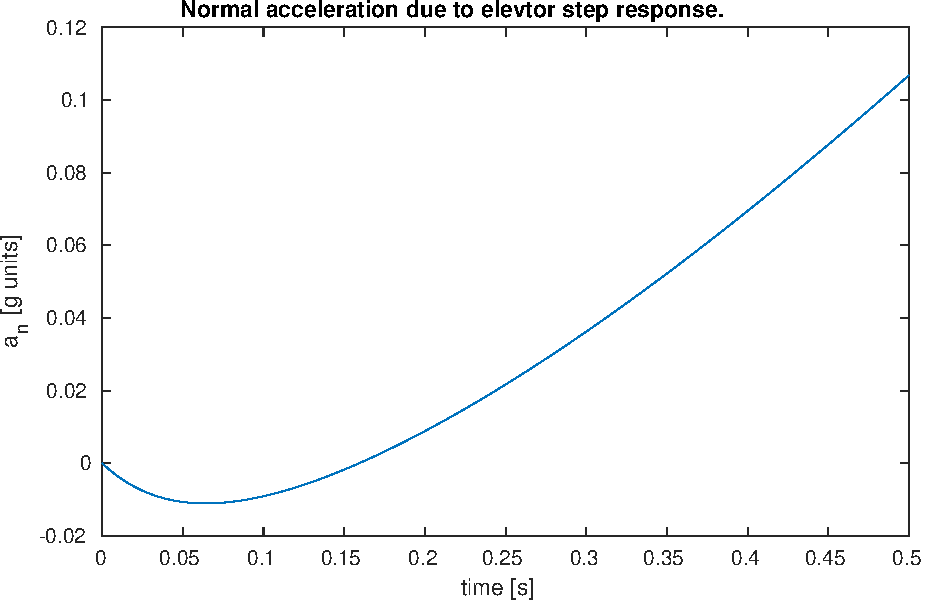
\includegraphics[width=0.6\textwidth]{figures/an_elev_step}
    \label{fig:an_elev_step}
    \caption{Normal acceleration after a negative step input on the elevator.}
\end{figure}

Repeating the simulation for increasing values of $x_a$ shows that the zero moves away from the origin indicating that its influence becomes less dominant. When $x_a=5.9$ the zero has moved to the left side of the imaginary axis and the non-minimum-phase behavior disappears. Since the value of the zero is significantly larger than that the other zeros and poles, its motion is negligible. Increasing $x_a$ further moves the zero closer to origin and its motion reappears, this time in the direction of the reference signal.

\begin{figure}[h]
    \centering
    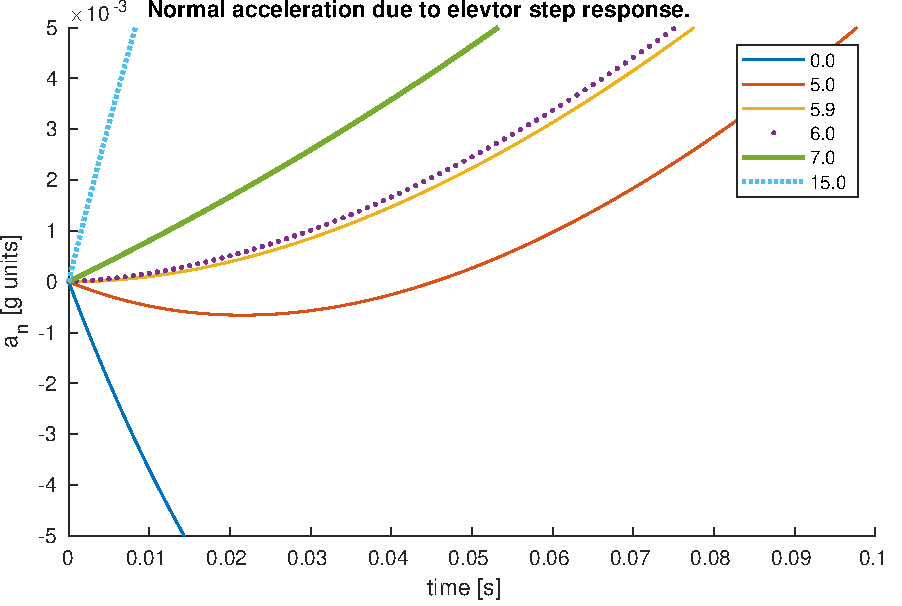
\includegraphics[width=0.6\textwidth]{figures/an_elev_step_mult}
    \caption{Normal acceleration after a negative step input on the elevator for different values of $x_a=5.9$.}
    \label{fig:an_elev_step_mult}
\end{figure}

One property of the \emph{instantaneous center of rotation} is that the linear accelerations at that point are the same as that of the aircraft. A point in front of it will accelerate upwards with a pitch up manoeuvre and a point behind it will accelerate downwards during the same manoeuvre. Thus based on the effects of moving $x_a$, it fair to conclude that the instantaneous center of rotation must be near $x=5.9$. Another way to arrive at the same conclusion is that the acceleration due to rotation is caused by the zero mentioned in the previous section since this is the only zero that changes significantly with $x_a$. Thus the instantaneous center of rotation will be at the location where this zero is infinitely far away from the origin.

The pilot should be placed at or after the instantaneous center of rotation ($x_a\geq5.9\ ft$), this is because if he is placed before, he will initially feel the aircraft moving into the opposite direction he is commanding it to and this might confuse the pilot resulting in him compensating for an error that is not there. This could make the combined human-aircraft system unstable or at least difficult to control.

It is important to place the accelerometer close a node of the most important fuselage bending moment. The reason is because, as the aircraft flies, loads and vibrations acting on the aircraft will make the fuselage bend. The nodes are locations where the displacements due to vibrations or bending are zero. Thus placing the accelerometer far away from a node, will result in the accelerometer measuring extra accelerations due to vibrations or bending. 

    \section{Open loop analysis}
\subsection{Longitudinal motion}
Reducing the state space system such that it only contains the states $\left \{ V_t, \alpha, \theta, q \right \}$ and input $\left \{ \delta_{el} \right \}$ results in the following matrices for the state space in Equation~\ref{eq:ssac}. $I_4$ is a 4x4 identity matrix and $0_{4,1}$ is a 4x1 zero matrix.

\begin{equation}
    \label{eq:sslon}
    \begin{aligned}
        A_{lon}&=\begin{bmatrix}
            -0.08894   &  -10.7   &   -32.17   & -3.977 \\
            -0.0005042 & -0.05167 & -3.989e-14 &   0.9792 \\
                    0 &        0 &          0 &        1 \\
            1.228e-18 &  -0.6256 &          0 &  -0.2485
        \end{bmatrix} &
        B_{lon}&=\begin{bmatrix}
            -0.07104 \\
            -0.0002308 \\
                    0 \\
            -0.01541 
        \end{bmatrix} \\\\
        C_{lon}&=I_4 &
        D_{lon}&=0_{4,1}
    \end{aligned}
\end{equation}

\begin{align}    
    \dot{x} &= A_{lon} \cdot x + B_{lon} \cdot u_{el} \nonumber\\
    y &= C_{lon} \cdot x + D_{lon} \cdot u_{el} \label{eq:ssac}
\end{align}

Analyzing the eigenvalues of the $A_{lon}$ matrix yields the following parameters for the inherent flight motions.

\begin{table}[h!]
    \centering
    \begin{tabular}{ r | c c c c c }
                     & Poles                            & $\zeta$        & $\omega_n$     & $P$           & $T_{1/2}$     \\ \hline \hline
        Short period & $\e{-1.53}{-1} + \e{7.62}{-1}i$ & $\e{1.97}{-1}$ & $\e{7.77}{-1}$ & $8.09$        & $4.43$        \\  
                     & $\e{-1.53}{-1} - \e{7.62}{-1}i$ & $\e{1.97}{-1}$ & $\e{7.77}{-1}$ & $8.09$        & $4.43$        \\ \hline
        Phugoid      & $\e{-4.17}{-2} + \e{1.23}{-1}i$ & $\e{3.22}{-1}$ & $\e{1.30}{-1}$ & $\e{4.82}{1}$ & $\e{1.56}{1}$ \\   
                     & $\e{-4.17}{-2} - \e{1.23}{-1}i$ & $\e{3.22}{-1}$ & $\e{1.30}{-1}$ & $\e{4.82}{1}$ & $\e{1.56}{1}$
    \end{tabular}
    \caption{Longitudinal eigenmotions poles, damping rations, natural frequencies, periods and time to half amplitude.}
\end{table}

The poles are the eigenvalues of $A_{lon}$ matrix, $\zeta$ the damping, $\omega_n$ the natural frequency, $P$ the oscillation period and $T_{1/2}$ the time to damp to half amplitude. These parameters are calculated from the poles $\lambda =\xi \pm \eta i$ using the following equations.

\begin{align}
    \omega_n&=\left | \lambda\right | \\
    \zeta&=-\frac{\xi}{\omega_n} \\
    P&=\frac{2\pi}{\omega_n} \\
    T_{1/2}&=P \cdot \frac{\ln{2}}{2 \pi} \cdot \frac{\sqrt{1-\zeta^2}}{\zeta}
\end{align}

Simulations are performed to get the time response for each motion in order to check whether the calculated parameters are correct. In order to do this check visually two elements are added to the figures. The first one are the \emph{period markers}. These are a set of vertical lines separated by the calculated period $P$ and aligned with the first peak.

The second element are one or two exponential decay functions in the form shown below.

\begin{equation}
    f(t) = C_1\left(\frac{1}{2}\right)^{\frac{t}{T_{1/2}}} + C_2
\end{equation}

Where $t$ is the time,and $C_1$ and $C_2$ are constants used to adjust the initial value. The result of this function reduces by half every $T_{1/2}$, thus it can be used to check whether the amplitude of the oscillations is reducing at the same rate. Figure~\ref{fig:ol_sp} shows the results of these simulations.

\begin{figure}[ht]
    \centering
    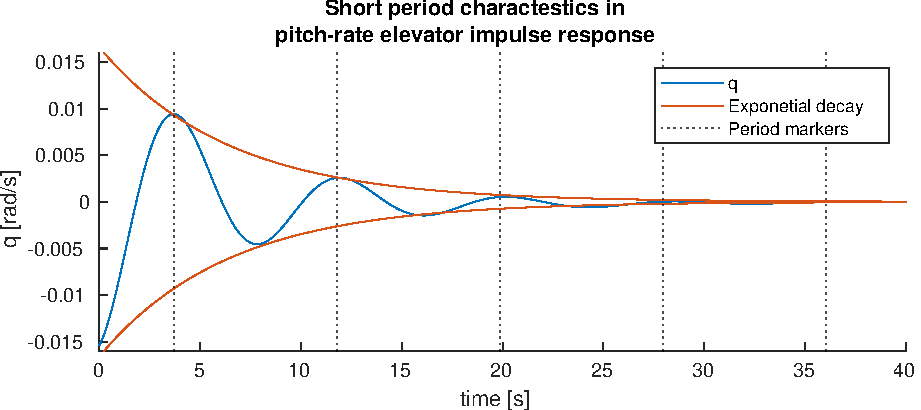
\includegraphics[width=0.6\textwidth]{figures/ol_sp}    
    \caption{Pitch-rate $q$ response during a short period oscillation, induced by a impulse elevator input.}
    \label{fig:ol_sp}
\end{figure}

\begin{figure}[ht]
    \centering
    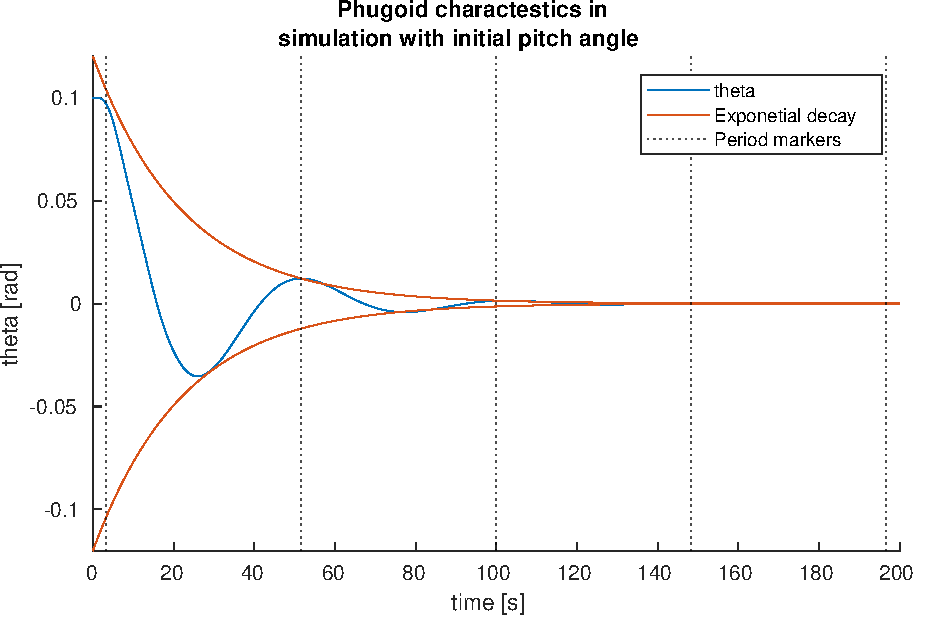
\includegraphics[width=0.6\textwidth]{figures/ol_ph}    
    \caption{Pitch angle $\theta$ response during a phugoid induced by an initial pitch angle of $\theta_0=0.1\ [rad]$}
    \label{fig:ol_ph}
\end{figure}

\subsection{Lateral motion}
Reducing the state space system such that it only contains the states $\left \{ \beta, \phi, p, r \right \}$ and inputs $\left \{ \delta_{a}, \delta_{r} \right \}$ results in the following matrices for the state space in Equation~\ref{eq:ssaclat}. $I_4$ is a 4x4 identity matrix and $0_{4,2}$ is a 4x2 zero matrix.


\begin{align*}
    A_{lat}&=\begin{bmatrix}
        -0.04905 & 0.08741 &  0.5803 & -0.8129 \\
               0 &       0 &       1 &  0.7105 \\
          -2.547 &       0 & -0.2594 &   0.151 \\
           -0.59 &       0 & 0.02607 & -0.1313
    \end{bmatrix} &
    B_{lat}&=\begin{bmatrix}
        4.181e-05 & 0.0001227 \\
                0 &         0 \\
          -0.0444 &  -0.00523 \\
         0.002184 & -0.004975 
    \end{bmatrix} \\\\
    C_{lat}&=I_4 &
    D_{lat}&=0_{4,2}
\end{align*}

\begin{align}    
    \dot{x} &= A_{lat} \cdot x + B_{lat} \cdot u_{el} \nonumber\\
    y &= C_{lat} \cdot x + D_{lat} \cdot u_{el} \label{eq:ssaclat}
\end{align}

The poles for this system are,
\begin{table}[h!]
    \centering
    \begin{tabular}{ c }
        Poles \\ \hline \hline
        $\e{-1.68}{-1}$ \\
        $\e{-1.68}{-1}$ \\
        $\e{-5.18}{-2}$ \\
        $\e{-5.18}{-2}$ \\
    \end{tabular}
    \caption{Lateral eigenmotion poles}
\end{table}

For the lateral motion is it expected to find two complex poles for the dutch roll and two real poles, one for the aperiodic roll and one for the spiral motion. However under the given flight conditions the linearization code fails and generates systems with four complex poles.

In order to continue with the assignment the flight conditions for the Accelerometer Position Analysis are used.

\begin{equation*}
    h_{apa} = 15000ft \qquad  V_{apa}=500ft/s
\end{equation*}

Linearising under these flight conditions results in the following,

\begin{align*}
    A_{lat}&=\begin{bmatrix}
        -0.2022 & 0.06414 & 0.07827 & -0.9919 \\
              0 &       0 &       1 &  0.0781 \\
         -22.92 &       0 &  -2.254 &  0.5408 \\
          6.005 &       0 & -0.0404 & -0.3146
    \end{bmatrix} &
    B_{lat}&=\begin{bmatrix}
        0.0001724 & 0.0005058 \\
                0 &         0 \\
          -0.4623 &   0.05686 \\
         -0.02437 &  -0.04687 
    \end{bmatrix} \\\\
    C_{lat}&=I_4 &
    D_{lat}&=0_{4,2}
\end{align*}

\begin{table}[h!]
    \centering
    \begin{tabular}{ r | c c c c c c }
                       & Poles                   & $\zeta$        & $\omega_n$     & $P$    & $T_{1/2}$     & $\tau$         \\ \hline \hline
        Dutch roll     & $\e{-3.20}{-1} + 2.74i$ & $\e{1.16}{-1}$ & $\e{7.77}{-1}$ & $2.28$ & $4.43$        &                \\  
                       & $\e{-3.20}{-1} - 2.74i$ & $\e{1.16}{-1}$ & $\e{7.77}{-1}$ & $2.28$ & $2.14$        &                \\ \hline
        Aperiodic roll & $2.12$                  &                &                &        & $\e{1.56}{1}$ & $\e{4.72}{-1}$ \\ \hline 
        Spiral         & $\e{-1.13}{-2}$         &                &                &        & $\e{1.56}{1}$ & $\e{8.88}{1}$
    \end{tabular}
    \caption{Lateral eigenmotions poles, damping rations, natural frequencies, periods, time to half amplitude and time constants.}
\end{table}

For the aperiodic eigenmotions, there is a new parameter $\tau$, the time constant and the time to damp to half amplitude $T_{1/2}$ is calculated differently.

\begin{align}
    \tau &= -\frac{1}{\lambda} \\
    T_{1/2} &= \ln{2}\ \tau
\end{align}

The results of these simulations are shown in the following figures. Despite being an aperiodic motions, the aperiodic roll and spiral results both contain oscillations. This is due to a less dominant dutch roll. To show this, Figure~\ref{fig:ol_apdsf} has the period markers with the period for the dutch roll added to it.

\begin{figure}[ht]
    \centering
    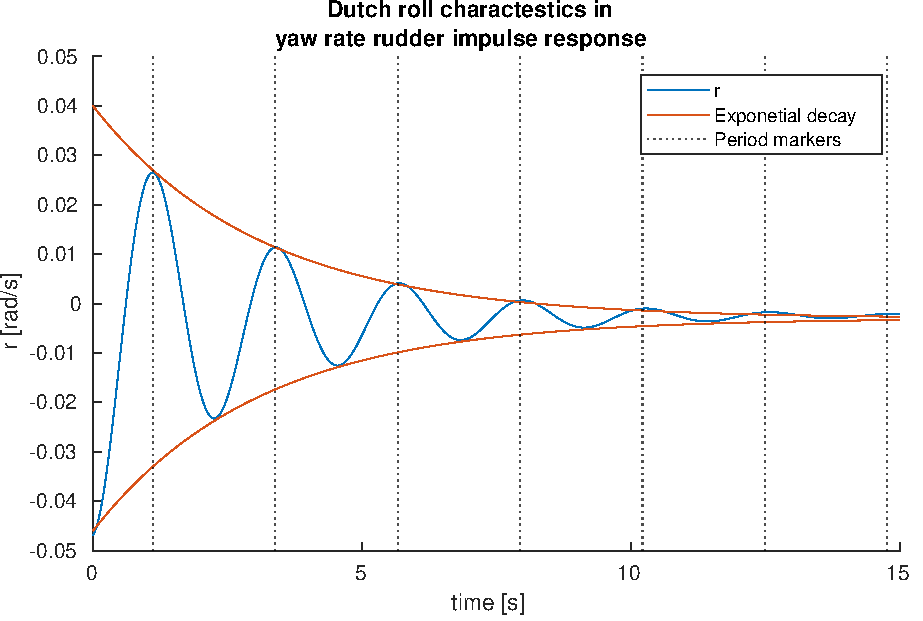
\includegraphics[width=0.6\textwidth]{figures/ol_dr}    
    \caption{Yaw rate $r$ response during a dutch roll induced by an impulse rudder input.}
    \label{fig:ol_dr}
\end{figure}

\begin{figure}[ht]
    \centering
    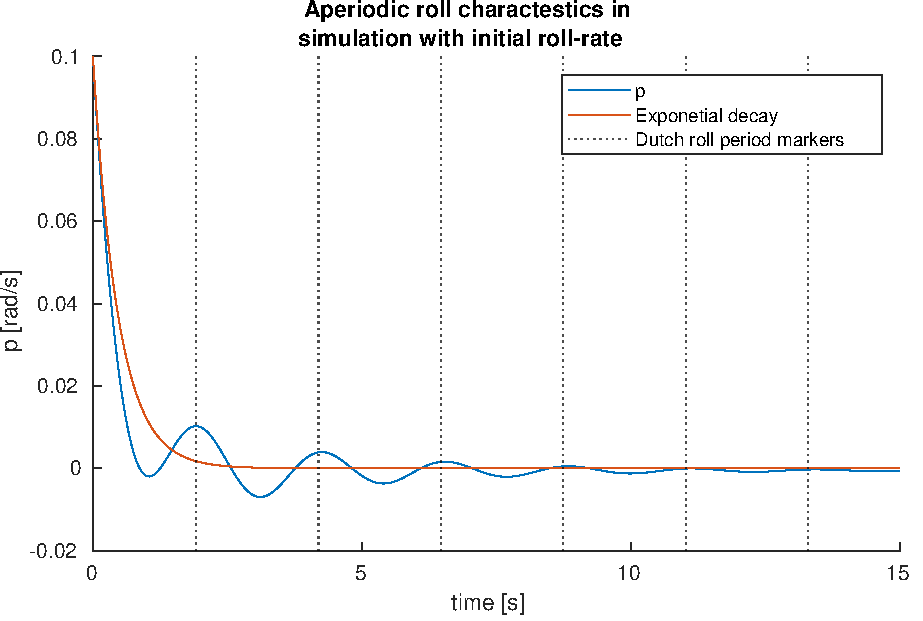
\includegraphics[width=0.6\textwidth]{figures/ol_ap}    
    \caption{Roll rate $p$ response during an aperiodic roll induced by an initial roll rate of $r_0=0.1\ 
    [rad\ s^{-1}]$}
    \label{fig:ol_apdsf}
\end{figure}

\begin{figure}[ht]
    \centering
    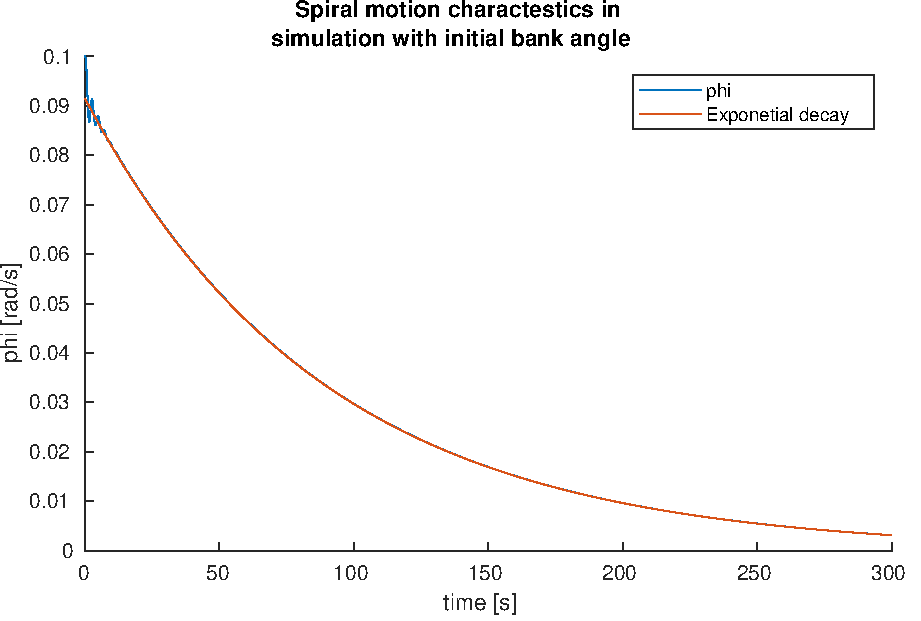
\includegraphics[width=0.6\textwidth]{figures/ol_si}    
    \caption{Bank angle $\phi$ response during a spiral motion induced by an initial bank angle of $\phi_0=0.1\ [rad]$}
    \label{fig:ol_si}
\end{figure}

\clearpage

    \section{Pitch rate command system}

Reducing the state space model in Equation~\ref{eq:sslon} by eliminating the velocity and pitch angle states result in the following model.

\begin{equation}
    \begin{aligned}
        A_{red}&=\begin{bmatrix}
            -0.05167 &   0.9792 \\
            -0.6256  & -0.2485
        \end{bmatrix} &
        B_{red}&=\begin{bmatrix}
            -0.0002308 \\
            -0.01541
        \end{bmatrix} \\\\
        C_{red}&=I_2 &
        D_{red}&=0_{2,1}
    \end{aligned}
\end{equation}

Simulating the step response for both models yields similar results. It is clear in the response of the full model that the short period is the dominant eigenmotion during the first few seconds. Since only the initial response of the system in relevant for the CAP and Gibson dropback criterion, it is fine to continue using the reduced model for the rest of the assignment.

\begin{figure}[ht]
    \centering
    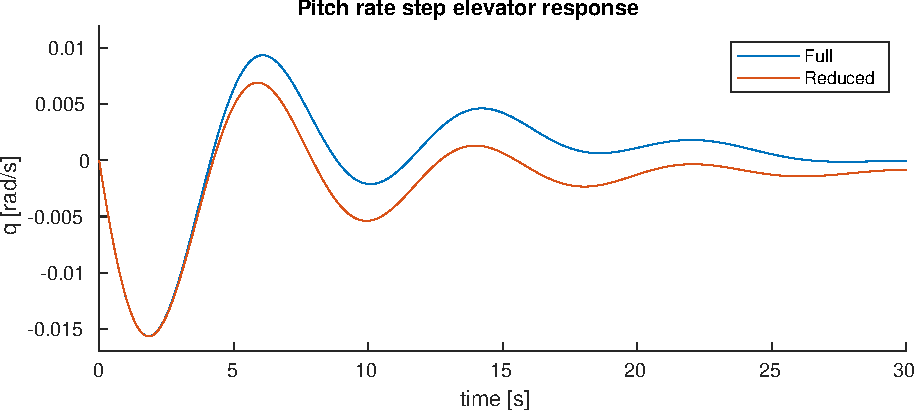
\includegraphics[width=0.6\textwidth]{figures/pc_acre_step.pdf}    
    \caption{Pitch rate elevator step response for both the full and reduced model.}
    \label{fig:pc_acre_step}
\end{figure}

A feedback loop is needed in order to satisfy the short period natural frequency and damping requirements. Figure~\ref{fig:pc_loop1} shows the control loop for solving this problem. The system $G$ is the open loop state space system and $K$ is the to be determined gain matrix.

\begin{figure}[ht]
    \centering
    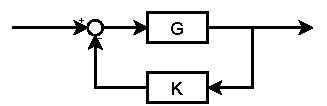
\includegraphics[width=0.4\textwidth]{figures/pc_loop1.pdf}    
    \caption{Feedback loop with gain in the loop.}
    \label{fig:pc_loop1}
\end{figure}

The build-in matlab function \texttt{place(...)} is used to calculate the gain $K_{reduced}$ using pole placement. The resulting gain is shown in Equation~\ref{eq:gaink}.

\begin{equation}
    \label{eq:gaink}
    K_{reduced}=\begin{bmatrix}
                    K_{\alpha} & K_q
                \end{bmatrix}
               =\begin{bmatrix}
                    -449.0440 & -151.8325
                \end{bmatrix}
\end{equation}

The new closed loop system matrix $A$ can then be calculated using Equation~\ref{eq:aclosed} and the rest of the matrices are the same as that of the open loop system. The new closed loop system can be found in Equation~\ref{eq:closedloopsystem}.

\begin{equation}
    \label{eq:aclosed}
    A_{closed} = A_{open}-B_{open}K
\end{equation}


\begin{equation}
    \label{eq:closedloopsystem}
    \begin{aligned}
        A_{closed}&=\begin{bmatrix}
            -0.1553 &  0.9442 \\
            -7.544  & -2.588 \\
        \end{bmatrix} &
        B_{closed}&=\begin{bmatrix}
            -0.0002308 \\
            -0.01541
        \end{bmatrix} \\\\
        C_{closed}&=I_2 &
        D_{closed}&=0_{2,1}
    \end{aligned}
\end{equation}

                                                                       
                                                                 

Calculating the damping and natural frequency of the closed loop system shows that the parameters match the required $\zeta=0.5$ and $\omega_n=0.03V\approx 2.74$
\begin{table}[h!]
    \centering
    \begin{tabular}{ c c c c c }
         Poles         & $\zeta$        & $\omega_n$ \\ \hline \hline
         $1.37 + 1.37i$ & $\e{5.00}{-1}$ & $2.74$     \\  
         $1.37 - 1.37i$ & $\e{5.00}{-1}$ & $2.74$     \\ \hline
    \end{tabular}
    \caption{Longitudinal eigenmotions poles, damping rations, natural frequencies, periods and time to half amplitude.}
\end{table}

If small angle approximations are assumed it is possible to calculate the angle of attack using the following equation.

\begin{equation}
    \alpha = \frac{w}{V}
\end{equation}

Here is $w$ the vertical airspeed component and V the total airspeed. Thus the angle of attack change in case of a vertical gust may be calculated by dividing the gust speed by the free stream velocity. This angle of attack may be passed as an initial condition to a simulation in order to observe the aircraft's behavior during such a gust. For a severe gust with $w=4.572\ [m\ s^{-1}]$ the initial angle of attack in the assigned flight condition is,

\begin{equation}
    \alpha_0=\frac{4.572\ [m\ s^{-1}]}{300\ [ft\ s^{-1}]}=\frac{4.572\ [m\ s^{-1}]}{91.44\ [m\ s^{-1}]} = 0.05\ [rad]
\end{equation}

The simulation results for both the open and closed loop systems using this initial condition and zero inputs is shown in Figure~\ref{fig:pc_vertgust}. As it can be seen the closed loop system quickly dampens the disturbance due the vertical gust, in contrast to the open loop system which continues oscillating significantly longer.

\begin{figure}[ht]
    \centering
    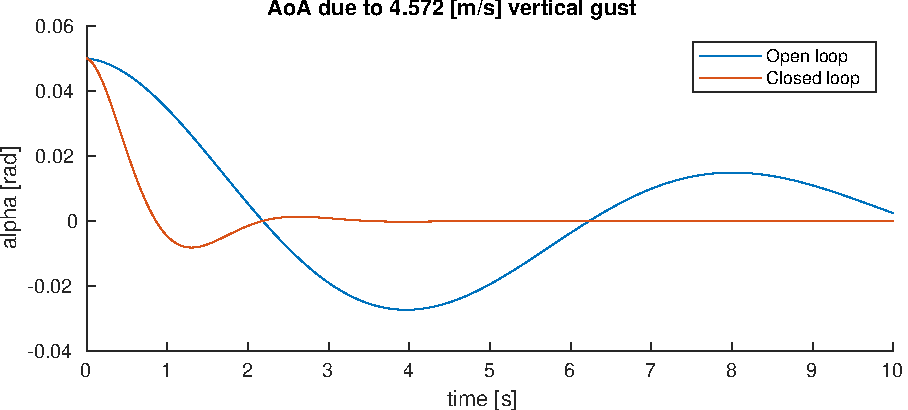
\includegraphics[width=0.6\textwidth]{figures/pc_vertgust.pdf}    
    \caption{Angle of attack during a $w=4.572\ [m\ s^{-1}]$ vertical gust for the open and closed loop systems.}
    \label{fig:pc_vertgust}
\end{figure}

The $T_{\theta_2}$ time constant cannot be modified by pole placement or by some other control loop structure. The reason is because it is located in the numerator of the transfer function and it's not possible to change the numerator using a feedback loop gain. 

Placing the lead-lag filter inside of the loop on the forward path will make it end up in both the numerator and denominator of the closed loop transfer function. Thus making it impossible to replace the zero without without changing the damping ratio and natural frequency of the closed loop system.

To modify $T_{\theta_2}$ a lead-lag prefilter can be placed before the closed loop system. The pole in the prefilter is used to cancel the current zero with $T_{\theta_2}$ in the closed loop, and the prefilter's zero end up in the overall transfer function, thus replacing the original zero.

\begin{equation}
    \frac{q(s)}{\delta_{el}(s)}=\frac{1+T_{\theta_2,new}}{1+T_{\theta_2,old}} \cdot
        \frac{k_q \left(1+T_{\theta_2,old}\right)}{
        s^2+2\zeta\omega_ns+\omega_n^2}
        =
        \frac{k_q \left(1+T_{\theta_2,new}\right)}{
        s^2+2\zeta\omega_ns+\omega_n^2}
\end{equation}

Even with the prefilter the controller will still not track the reference pitch rate signal properly, there will be a steady state error that needs to be compensated for. The reason is because the signal coming from the feedback loop is scaled by the gain $K$ and thus the reference signal needs to be scaled as well.

For this assignment the \texttt{rscale(...)} function which can be found at \cite{matlabrscale} is used. The final form of the precompensator is thus,

\begin{equation}
    N \cdot \frac{1+T_{\theta_2,new}}{1+T_{\theta_2,old}}
\end{equation}

Where $N$ is the scaling factor from \texttt{rscale(...)}.


% Category B: Those nonterminal Flight Phases that are normally accomplished using
% gradual maneuvers and without precision tracking, although accurate
% flight-path control may be required. Included in this Category are:

Figure~\ref{fig:pc_cap} shows the level 1 Control Anticipation Parameter criteria for Category B flight phases. According to \cite{milstd1797a}, Category B flights phases are normally accomplished using gradual maneuvers and without precision tracking, which includes cruise flight. As it can be seen, the controller satisfies the requirement.

\begin{equation}
    CAP=\frac{g\omega^2T_{\theta_2}}{V} \approx 0.1168
\end{equation}

\begin{figure}[ht]
    \centering
    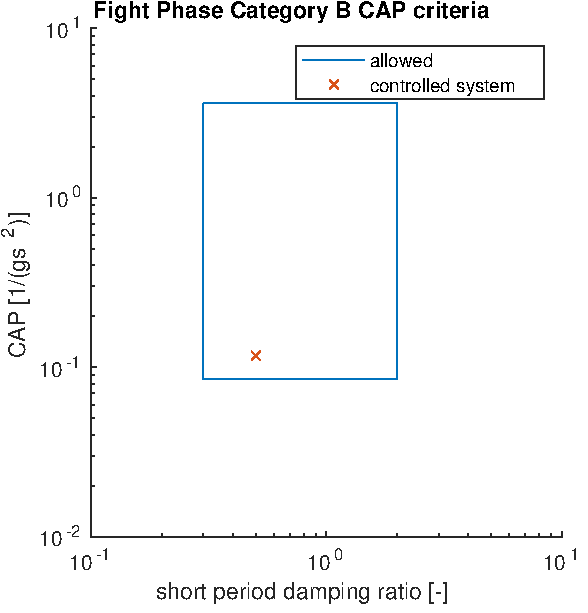
\includegraphics[width=0.4\textwidth]{figures/pc_cap.pdf}    
    \caption{Control Anticipation Parameter criteria for Category B flight phases and the location for the controlled system in the plot.}
    \label{fig:pc_cap}
\end{figure}

Figure~\ref{fig:pc_cap} shows the pitch rate and pitch angle step response of the controlled system. The maximum pitch rate $q_m$ and steady state value $q_s$ are marked in the plot. 
\begin{figure}[ht]
    \centering
    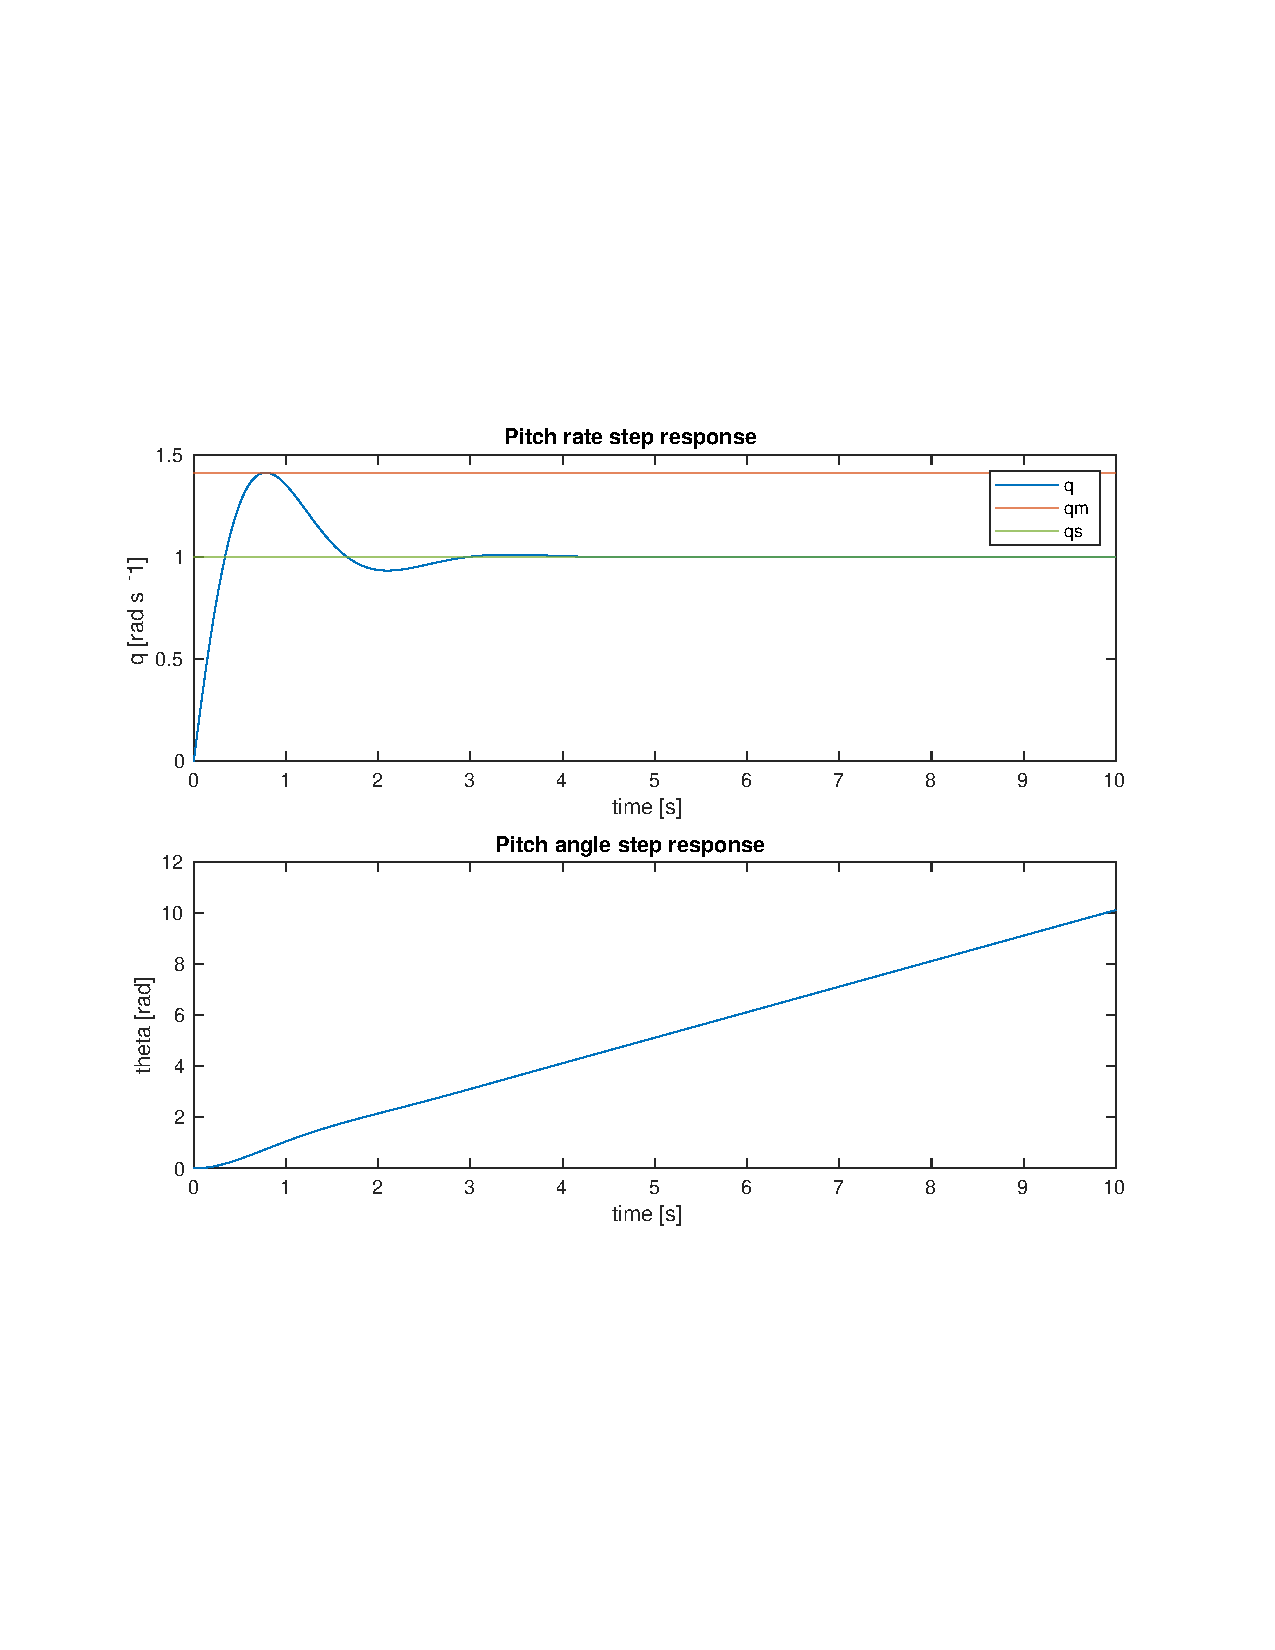
\includegraphics[width=0.8\textwidth]{figures/pc_pitch_resp.pdf}    
    \caption{Pitch rate and pitch angle step response of the controlled system.}
    \label{fig:pc_pitch_resp}
\end{figure}



Figure~\ref{fig:pc_cap} shows the satisfactory range of values to meet the Gibson dropback criterion. As it can be seen the controlled system satisfies the criteria.
\begin{align}
    \label{eq:gibvals}
    \frac{DB}{q_s} &= T_{\theta_2} - \frac{2\zeta_{sp}}{\omega_{n_{sp}}} \approx 0.1099 \\
    \frac{q_m}{q_s} &= \frac{1.4126}{1} = 1.4126
\end{align}

\begin{figure}[ht]
    \centering
    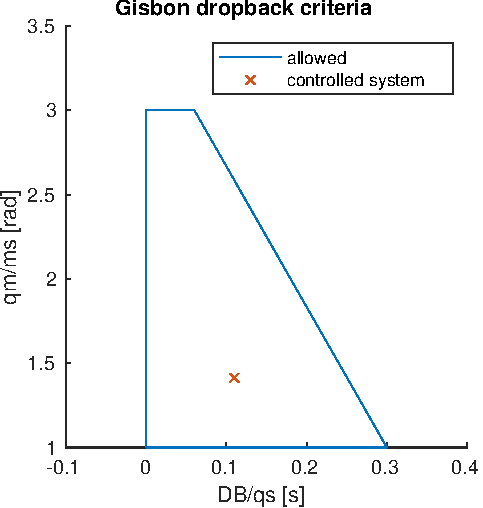
\includegraphics[width=0.4\textwidth]{figures/pc_gib.pdf}    
    \caption{Pitch rate and pitch angle step response of the controlled system.}
    \label{fig:pc_gib}
\end{figure}



\clearpage


    \newpage
    \printbibliography

\end{document}
